\section{Overview}
\label{sec:joint-overview}

Joint segmentation and tracking describes a method that breaks the fixed border between the
segmentation phase and the tracking phase in a
tracking-by-assignment~(\cref{sec:tracking-by-assignment}). More precisely, at first an
oversegmentation of the raw data is generated such that each foreground \emph{segment} contains not
more than a single cell. On the contrary, each cell in the raw data may consist of multiple
segments. The tracking model then decides whether a segment belongs to foreground or background and
groups segments into cell objects.

For clarity and an unambiguous definition of the joint segmentation and tracking, we first define
notational conventions that will be used throughout this chapter.
\begin{mydef}
    \label{def:joint-segment}
    A \emph{segment} or \emph{superpixel/-voxel} is the smallest unit in a segmentation. It is part of or a complete foreground
    object.
\end{mydef}

\begin{mydef}
    \label{def:joint-region}
    A \emph{region} is either a single segment or the union of two neighboring regions. Thus, the
    segments form a subset of all regions. Neighborhood relationships can be visualized in a
    \emph{region adjacency graph}.
\end{mydef}

\begin{mydef}
    \label{def:joint-conflict}
    Two regions \emph{contradict} each other if the intersection of their contained segments is not
    the empty set. In other words, they form a \emph{conflict}. These conflicts can be visualized in
    a conflict graph.
\end{mydef}

\begin{mydef}
    \label{def:joint-connected-component}
    A \emph{connected component} contains all segments that are connected by a path in the region
    adjacency graph.
\end{mydef}
Note that, by definition, a connected component is also a region. 

\begin{mydef}
    \label{def:joint-cardinality}
    The \emph{cardinality} of a region $r$ is the number of segments that the region consists of. It
    is denoted by $|r|$.
\end{mydef}
In the context of a conflict graph, the cardinality of a region $r$ is the number of maximal
cliques~(\cref{def:clique}) or \emph{``conflict sets''} in the conflict graph that contain region
$r$. In general, each conflict set contains exactly one segment, which can be used as an identifier
of the conflict set. These definitions are subsumed in \cref{tab:joint-definitions} with
illustrative visualizations.  \newlength\tablenormaltext
\settototalheight\tablenormaltext{\parbox{\linewidth}{Raw Data}}
\begin{table}
    \centering
    \scalebox{0.85}{
        \def\arraystretch{0.5}
% \setlength{\tabcolsep}{1pt}
\begin{tabularx}{\textwidth}{p{5cm}l}
    \toprule
    Definition  & Visualization \\ \midrule
    % \begin{minipage}[t]{0.15\linewidth}\small\vspace{-53pt}{$\begin{aligned}t&=75\\\id&=446\\
    %         k&=3\end{aligned}$}\end{minipage}&
    % \raisebox{-0.8\height{\includegraphics...}}
    Raw Data (original image \& enhanced contrast) &
    \raisebox{\tablenormaltext-\height}{
        
\includegraphics[width=0.18\textwidth]{images/joint/overseg/75/02/raw.png}}
    \raisebox{\tablenormaltext-\height}{
        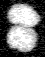
\includegraphics[width=0.18\textwidth]{images/joint/overseg/75/02/raw_contrast.png}} \\ & \\
    Segment&
    \raisebox{\tablenormaltext-\height}{
        
\includegraphics[width=0.18\textwidth]{images/joint/overseg/75/02/colored00.png}} \\ & \\
    Region (with ids) &
    \raisebox{\tablenormaltext}{
        \begin{tikzpicture}[baseline=(image1.north)]
            \node[anchor=south west,inner sep=0] (image1) {
                
\includegraphics[width=0.18\textwidth]{images/joint/overseg/75/02/colored00.png}};
            \begin{scope}[x={(image1.south east)},y={(image1.north west)}]
                \node[region_id] at (0.4, 0.75) {\huge{$1$}};
                \node[region_id] at (0.65, 0.7) {\huge{$2$}};
                \node[region_id] at (0.5, 0.32) {\huge{$3$}};
                % helpers
                % http://tex.stackexchange.com/questions/9559/drawing-on-an-image-with-tikz/9561
                % \draw[help lines,xstep=.1,ystep=.1] (0,0) grid (1,1);
                % \foreach \x in {0,2,...,8} { \node [anchor=north] at (\x/10,0) {0.\x}; }
                % \foreach \y in {0,2,...,8} { \node [anchor=east] at (0,\y/10) {0.\y}; }
            \end{scope}
        \end{tikzpicture}}
    \raisebox{\tablenormaltext}{
        \begin{tikzpicture}[baseline=(image2.north)]
            \node[anchor=south west,inner sep=0] (image2) {
                
\includegraphics[width=0.18\textwidth]{images/joint/overseg/75/02/colored01_all.png}};
            \begin{scope}[x={(image1.south east)},y={(image2.north west)}]
                \node[region_id] at (0.53, 0.73) {\huge{$4$}};
                \node[region_id] at (0.5, 0.32) {\huge{$3$}};
            \end{scope}
        \end{tikzpicture}}
    \raisebox{\tablenormaltext}{
        \begin{tikzpicture}[baseline=(image3.north)]
            \node[anchor=south west,inner sep=0] (image3) {
                
\includegraphics[width=0.18\textwidth]{images/joint/overseg/75/02/colored02.png}};
            \begin{scope}[x={(image1.south east)},y={(image3.north west)}]
                \node[region_id] at (0.5, 0.32) {\huge{$5$}};
            \end{scope}
        \end{tikzpicture}}
    \\ & \\
    Connected Component&
    \raisebox{\tablenormaltext-\height}{
        
\includegraphics[width=0.18\textwidth]{images/joint/overseg/75/02/colored02.png}} \\ & \\
    Region Adjacency Graph (edges indicate adjacency)&
    \raisebox{\tablenormaltext}{
        \begin{tikzpicture}[baseline=(r1.north)]
            \node[region_graph] (r1) {$1$};
            \node[region_graph, right=of r1.west] (r2) {$2$};
            \node[region_graph, below=of r1.north] (r3) {$3$};
            \node[region_graph, right=of r3.west] (r4) {$4$};
            \node[region_graph, right=of r2.west] (r5) {$5$};
            \path[region_edge] (r1) edge (r2);
            \path[region_edge] (r2) edge (r3);
            \path[region_edge] (r3) edge (r4);
        \end{tikzpicture}}
    \\ & \\
    Conflict Graph (edges indicate conflicts)&
    \raisebox{\tablenormaltext}{
        \begin{tikzpicture}[baseline=(r1.north)]
            \node[conflict_graph] (r5) {$5$};
            \node[conflict_graph, right=of r5.west] (r1) {$1$};
            \node[conflict_graph, below=of r5.north] (r2) {$2$};
            \node[conflict_graph, right=of r2.west] (r4) {$4$};
            \node[conflict_graph, left=of r2.east] (r3) {$3$};
            \path[conflict_edge] (r5) edge (r1);
            \path[conflict_edge] (r5) edge (r2);
            \path[conflict_edge] (r5) edge (r3);
            \path[conflict_edge] (r5) edge (r4);
            \path[conflict_edge] (r4) edge (r1);
            \path[conflict_edge] (r4) edge (r2);
        \end{tikzpicture}}
    \\ & \\
    \bottomrule
    
\end{tabularx}
\def\arraystretch{1.0}


%%% Local Variables: 
%%% mode: latex
%%% TeX-master: "../../main"
%%% End: 

    }
    \caption[Notational conventions in the joint segmentation and tracking]{Notational conventions in the joint segmentation and
        tracking with visualizations on a cell from data set
        C~(\cref{subsubsec:gmm-data-c}). Segments and regions are color coded for better
        distinguishability. In case of overlapping regions, multiple images are added.}
    \label{tab:joint-definitions}
\end{table}

With the definitions at hand, we now give a brief digest of our new joint segmentation and tracking
method. First, we obtain a possibly undersegmented partition of the raw data into foreground and
background. At this stage, a foreground connected component may contain more than one single
cell. Moreover, the segmentation aims to include all cells in the data into foreground, regardless
of possibly merged objects~(\cf \cref{fig:joint-underseg-mergers}). Then, another segmentation
algorithm is applied to the foreground mask of the data with the intent to
oversegment~(\cref{sec:joint-oversegmentation}). This divides the foreground into segments from which an
initial region adjacency graph is created. Next, regions are gradually merged to form a richer set of
\emph{segmentation hypotheses}. The \emph{tracking hypotheses graph} is then formulated on the
connected component in the image. An edge connecting two nodes $n_1$, $n_2$ in this graph means that
any pair of two regions, one from $n_1$ and one from $n_2$, is a potential tracking
assignment. Finally, a factor graph~(\cref{sec:joint-graphical-model}) is built on top of the
hypotheses graph. The factor graph incorporates prior belief on configurations inferred by local
classifiers~(\cref{sec:joint-classifiers}) as well as restrictions on possible assignments and
segmentation hypotheses that are defined by the conflict graph and the requirements of cell
tracking. Then, inference on this factor graph yields the optimal tracking solution. This procedure
is illustrated in \cref{fig:joint-pipeline}.

\begin{figure}
    \centering
    \scalebox{0.8}{
        \begin{tikzpicture}
    \newcommand{\distancebetween}{20}
    \newcommand{\shiftdistance}{100}
    \newcommand{\scalingfactor}{0.12}
    \newcommand{\halfscalingfactor}{\scalingfactor}
    
    \begin{scope}
        \begin{scope}[baseline=(raw2)]
    \begin{scope}[yshift=\distancebetween,
        every node/.append style={yslant=0.5,xslant=-1},
        yslant=0.5,xslant=-1]
        \node[inner sep=0, label={[xshift=5]above:{}}] (raw1) {
            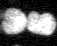
\includegraphics[width=\scalingfactor\textwidth]{images/joint/pipeline/78_raw_crop_enhanced.png}
        };
    \end{scope}
    \begin{scope}[every node/.append style={yslant=0.5,xslant=-1},yslant=0.5,xslant=-1]
        \begin{pgfonlayer}{bglower}
            \node[inner sep=0, label={[xshift=15]above:{}}] (raw2) {
                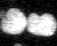
\includegraphics[width=\scalingfactor\textwidth]{images/joint/pipeline/79_raw_crop_enhanced.png}
            };
        \end{pgfonlayer}
    \end{scope}
    \coordinate (base1) at (raw2.north west |- raw2.south west);
    \coordinate (base2) at (raw2.south east |- raw2.south west);
    % \draw [pllbl]
    % (base1) -- (base2) node[black,midway,yshift=-0.6cm]
    % {Raw Data};
    \path let \p1 = (base1.west), \p2 = (base2.east) in
    node[pllbltxt, minimum width=\x2-\x1] (labelraw) at ($(base1)!0.5!(base2)$)
    {\phantom{g}Raw Data\phantom{g}};
    \begin{pgfonlayer}{bglower}
        \path[threed] (raw2.south east) -- (raw1.south east);
        \path[threed] (raw2.north east) -- (raw1.north east);
        \path[threed] (raw2.south west) -- (raw1.south west);
        \path[threed] (raw2.north west) -- (raw1.north west);
    \end{pgfonlayer}
\end{scope}

%%% Local Variables: 
%%% mode: latex
%%% TeX-master: "../../../main"
%%% End: 

        % \node[ultra thick, left=of raw1,yshift=5mm] {$t\phantom{+1}$};
        % \node[ultra thick, left=of raw2,yshift=5mm] {$t+1$};
        \begin{scope}[xshift=\shiftdistance, baseline=(seg2)]
    \begin{scope}[yshift=\distancebetween,
        every node/.append style={yslant=0.5,xslant=-1},
        yslant=0.5,xslant=-1]
        \node[inner sep=0, label={[xshift=5]above:{}}] (seg1) {
            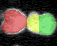
\includegraphics[width=\scalingfactor\textwidth]{images/joint/pipeline/78_seg_crop.png}
        };
    \end{scope}
    \begin{scope}[every node/.append style={yslant=0.5,xslant=-1},yslant=0.5,xslant=-1]
        \begin{pgfonlayer}{bglower}
            \node[inner sep=0, label={[xshift=15]above:{}}] (seg2) {
                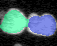
\includegraphics[width=\scalingfactor\textwidth]{images/joint/pipeline/79_seg_crop.png}
            };
        \end{pgfonlayer}
    \end{scope}
    \coordinate (base1) at (seg2.north west |- seg2.south west);
    \coordinate (base2) at (seg2.south east |- seg2.south west);
    % \draw [pllbl]
    % (base1) -- (base2) node[black,midway,yshift=-0.6cm]
    % {Initial Oversegmentation};
    \path let \p1 = (base1.west), \p2 = (base2.east) in
    node[pllbltxt, minimum width=\x2-\x1] (labelseg) at ($(base1)!0.5!(base2)$) {Oversegmentation};
    \begin{pgfonlayer}{bglower}
        \path[threed] (seg2.south east) -- (seg1.south east);
        \path[threed] (seg2.north east) -- (seg1.north east);
        \path[threed] (seg2.south west) -- (seg1.south west);
        \path[threed] (seg2.north west) -- (seg1.north west);
    \end{pgfonlayer}
\end{scope}

%%% Local Variables: 
%%% mode: latex
%%% TeX-master: "../../../main"
%%% End: 

        \begin{scope}[xshift=2*\shiftdistance, baseline=(cc2)]
    \begin{scope}[yshift=\distancebetween,
        every node/.append style={yslant=0.5,xslant=-1},
        yslant=0.5,xslant=-1]
        \node[inner sep=0, label={[xshift=5]above:{}}] (merge1) {
            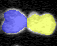
\includegraphics[width=\halfscalingfactor\textwidth]{images/joint/pipeline/78_merge_crop.png}
        };
        \node[inner sep=0,xshift=47,yshift=-47, label={[xshift=5]above:{}}] (cc1) {
            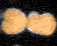
\includegraphics[width=\halfscalingfactor\textwidth]{images/joint/pipeline/78_cc_crop.png}
        };
    \end{scope}
    \begin{scope}[every node/.append style={yslant=0.5,xslant=-1},yslant=0.5,xslant=-1]
        \begin{pgfonlayer}{bglower}
            \node[inner sep=0, label={[xshift=15]above:{}},rectangle,thin,draw] (merge2) {
                \phantom{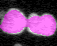
\includegraphics[width=\scalingfactor\textwidth]{images/joint/pipeline/79_cc_crop.png}}
            };
            \node[xshift=47,yshift=-47,inner sep=0, label={[xshift=15]above:{}}] (cc2) {
                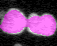
\includegraphics[width=\scalingfactor\textwidth]{images/joint/pipeline/79_cc_crop.png}
            };
        \end{pgfonlayer}
    \end{scope}
    \coordinate (base1) at (merge1.north west |- cc2.south west);
    \coordinate (base2) at (cc1.south east |- cc2.south west);
    % \draw [pllbl]
    % (base1) -- (base2) node[black,midway,yshift=-0.6cm]
    % {Region Merging};
    \path let \p1 = (base1.west), \p2 = (base2.east) in
    node[pllbltxt, minimum width=\x2-\x1] (labelmerging) at ($(base1)!0.5!(base2)$) {Region Merging};
    \begin{pgfonlayer}{bglower}
        \path[threed] (merge2.south east) -- (merge1.south east);
        \path[threed] (merge2.north east) -- (merge1.north east);
        \path[threed] (merge2.south west) -- (merge1.south west);
        \path[threed] (merge2.north west) -- (merge1.north west);

        \path[threed] (cc2.south east) -- (cc1.south east);
        \path[threed] (cc2.north east) -- (cc1.north east);
        \path[threed] (cc2.south west) -- (cc1.south west);
        \path[threed] (cc2.north west) -- (cc1.north west);
    \end{pgfonlayer}
\end{scope}

%%% Local Variables: 
%%% mode: latex
%%% TeX-master: "../../../main"
%%% End: 

        \begin{pgfonlayer}{background}
            \node[plbg, fit=(raw2.south west) (raw2.north west)
            (raw1.north east) (cc1.south east) (labelraw)] (bg1) {};
        \end{pgfonlayer}
        \draw[arrows=->, ultra thick, transform canvas={xshift=-15}] (bg1.north west) -- (bg1.south
        west) node[midway, xshift=-7] (t1) {\large{$t$}};
    \end{scope}
    \begin{scope}[yshift=-7.5*\distancebetween, xshift=100]
        \begin{scope}
    \begin{scope}[yshift=1.5*\distancebetween,
        every node/.append style={yslant=0.5,xslant=-1},
        yslant=0.5,xslant=-1]
        \node[inner sep=0] (image1) {
            \phantom{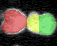
\includegraphics[width=\scalingfactor\textwidth]{images/joint/pipeline/78_seg_crop.png}}
        };
        \begin{pgfonlayer}{upper}
            \begin{scope}[every node/.append style={scale=0.7}]
                \node[fg_det, label={[font=\tiny]center:$X_1^t$}] (a1) at (image1.south east) {};
                \node[fg_det, label={[font=\tiny]center:$X_2^t$}] (a2) at ($(image1.south east)!0.5!(image1.north east)$) {};
                \node[fg_det, label={[font=\tiny]center:$X_3^t$}] (a3) at (image1.north east) {};
                \node[fg_det, label={[font=\tiny]center:$X_5^t$}] (a5) at ($(image1.south west)!0.5!(image1.north west)$) {};
                \node[fg_det, label={[font=\tiny]center:$X_4^t$}] (a4) at ($(a3)!0.5!(a5)$) {};
            \end{scope}
            \begin{scope}[every node/.append style={scale=0.5}]
                \node[conflict,yshift=-5] (c1) at ($(a1)!0.5!(a5)$) {};
                \node[conflict, right=of a3, xshift=-20, yshift=20] (c2) {};
                \node[conflict, yshift=-20] (c3) at (a4) {};
                \node[count, yshift=-20] (c4)  at ($(a2)!0.5!(a4)$) {};
                
                \path[count] (a1) edge (c4);
                \path[count] (a2) edge (c4);
                \path[count] (a3.south) edge (c4);
                \path[count] (a4) edge (c4);
                \path[count] (a5) edge[bend right=20] (c4);
                
                \path[conflict] (a5) edge[bend right=10] (c1);
                \path[conflict] (a1) edge (c1);

                \path[conflict] (a2) edge (c2);
                \path[conflict] (a4) edge[bend left=100] (c2);
                \path[conflict] (a5) edge[bend left=95] coordinate[pos=0.65](helpercoord1) (c2);

                \path[conflict] (a3) edge[bend left=10] (c3);
                \path[conflict] (a4) edge (c3);
                \path[conflict] (a5) edge (c3);
            \end{scope}
        \end{pgfonlayer}
        \begin{pgfonlayer}{bgupper}
            \node[rectangle, color=black,thick, fill=hypothesesbackground!30, opacity=0.8, draw=black,
            fit=(a1) (c2) (a5) (helpercoord1), inner sep=2, opacity=0.8, label={[xshift=5]above:{}}]
            (bgup) {};
        \end{pgfonlayer}
    \end{scope}
    \begin{scope}[every node/.append style={yslant=0.5,xslant=-1},yslant=0.5,xslant=-1]
        \node[inner sep=0] (image2) {
            \phantom{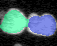
\includegraphics[width=\scalingfactor\textwidth]{images/joint/pipeline/79_seg_crop.png}}
        };
        \begin{pgfonlayer}{bglower}
            \node[rectangle, color=black,thick, fill=hypothesesbackground!30, opacity=0.8, draw=black,
            fit=(a1) (c2) (a5) (helpercoord1), inner sep=2, opacity=0.8, shift=($(image2) - (image1)$), label={[xshift=15]above:{}}]
            (bglow) {};
        \end{pgfonlayer}
        \begin{pgfonlayer}{lower}
            \begin{scope}[every node/.append style={scale=0.7}]
                \node[fg_det, label={[font=\tiny]center:$X_6^{t+1}$}] (b1) at (image2.south east) {};
                \node[fg_det, label={[font=\tiny]center:$X_7^{t+1}$}] (b2) at (image2.north east) {};
                \node[fg_det, label={[font=\tiny]center:$X_8^{t+1}$}] (b3) at ($(image2.south west)!0.5!(image2.north west)$) {};
            \end{scope}
            \begin{scope}[every node/.append style={scale=0.5}]
                \path[conflict] (b1) edge (b3);
                \path[conflict] (b3) edge (b2);
                \node[conflict] (c1) at ($(b1)!0.5!(b3)$) {};
                \node[conflict] (c2) at ($(b2)!0.5!(b3)$) {};
                \node[count] (c3) at ($(b1)!0.5!(b2)!0.3!(b3)$) {};
                \path[count] (b1) edge (c3);
                \path[count] (b2) edge (c3);
                \path[count] (b3) edge (c3);
            \end{scope}
        \end{pgfonlayer}
    \end{scope}
    \begin{pgfonlayer}{transition}
        \begin{scope}[every node/.append style={scale=0.6}]
            \node[fg_tra,label={[font=\tiny]center:$Y_{1,6}^t$},xshift=30] (trans1) at ($(a1)!0.55!(b1)$) {};
        \end{scope}
        \begin{scope}[every node/.append style={scale=0.2}]
            \node[transfac] (out) at ($(a1.center)!0.5!(trans1)$) {};
            \node[transfac] (in) at ($(b1.center)!0.5!(trans1)$) {};
            \path[transfac] (a1) edge (out.center);
            \path[transfac] (out) edge (trans1);
            \path[transfac] (trans1) edge (in);
            \path[transfac] (in) edge (b1.center);
        \end{scope}
    \end{pgfonlayer}
    \coordinate (base1) at (bglow.north west |- bglow.south west);
    \coordinate (base2) at (bglow.south east |- bglow.south west);
    % \draw [pllbl] (base1) -- (base2) node[black,midway,yshift=-0.6cm] {Factor Graph};
    \path let \p1 = (base1.west), \p2 = (base2.east) in
    node[pllbltxt, minimum width=\x2-\x1] (labelgraph) at ($(base1)!0.5!(base2)$) {Factor Graph};
    \begin{pgfonlayer}{bglower}
        \path[threed] (bglow.south east) -- (bgup.south east);
        \path[threed] (bglow.north east) -- (bgup.north east);
        \path[threed] (bglow.south west) -- (bgup.south west);
        \path[threed] (bglow.north west) -- (bgup.north west);
    \end{pgfonlayer}
\end{scope}

%%% Local Variables: 
%%% mode: latex
%%% TeX-master: "../../../main"
%%% End: 

        % \node[ultra thick, left=of raw1,yshift=5mm] {$t\phantom{+1}$};
        % \node[ultra thick, left=of raw2,yshift=5mm] {$t+1$};
        \begin{scope}[xshift=1.3*\shiftdistance]
    \begin{scope}[yshift=\distancebetween,
        every node/.append style={yslant=0.5,xslant=-1},
        yslant=0.5,xslant=-1]
        \node[inner sep=0, label={[xshift=5]above:{}}] (res1) {
            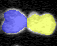
\includegraphics[width=\scalingfactor\textwidth]{images/joint/pipeline/78_res_crop.png}
        };
    \end{scope}
    \begin{scope}[every node/.append style={yslant=0.5,xslant=-1},yslant=0.5,xslant=-1]
        \begin{pgfonlayer}{bglower}
            \node[inner sep=0, label={[xshift=15]above:{}}] (res2) {
                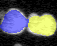
\includegraphics[width=\scalingfactor\textwidth]{images/joint/pipeline/79_res_crop.png}
            };
        \end{pgfonlayer}
    \end{scope}
    \coordinate (base1) at (res2.north west |- bglow.south west);
    \coordinate (base2) at (res2.south east |- bglow.south west);
    % \draw (base1) rectangle[pllbltxt, yshift=-10] (base2);%  {Tracking Result};
    \path let \p1 = (base1.west), \p2 = (base2.east) in
    node[pllbltxt, minimum width=\x2-\x1]  (labelres) at ($(base1)!0.5!(base2)$) {Tracking Result};
    \begin{pgfonlayer}{bglower}
        \path[threed] (res2.south east) -- (res1.south east);
        \path[threed] (res2.north east) -- (res1.north east);
        \path[threed] (res2.south west) -- (res1.south west);
        \path[threed] (res2.north west) -- (res1.north west);
    \end{pgfonlayer}
\end{scope}

%%% Local Variables: 
%%% mode: latex
%%% TeX-master: "../../../main"
%%% End: 

        \begin{pgfonlayer}{background}
            \node[plbg, fit=(bglow.south west) (bglow.north west)
            (bgup.north east) (res1.south east) (labelres.south)] (bg2) {};
        \end{pgfonlayer}
        \draw[arrows=->, ultra thick, transform canvas={xshift=-15}] (bg2.north west) -- (bg2.south
        west) node[midway, xshift=-7] (t2) {\large{$t$}};
    \end{scope}

    \begin{pgfonlayer}{background}
        \coordinate[xshift=0mm,left=of t1] (hawaii);
        \coordinate[right=of bg1.east,xshift=0mm] (coordeast);
        % \coordinate[below right=of bg1.south east,yshift=-5mm] (coordsouth);
        \coordinate (helper) at ($(bg1.south)!0.5!(bg2.north)$);
        \coordinate (coordsoutheast) at (coordeast |- helper);
        \coordinate[left=of t2.west,xshift=0mm] (coordwestwest);
        \coordinate[xshift=15mm] (coordwest) at (coordwestwest);
        \coordinate (coordsouthwest) at (coordwestwest |- helper);
        \path[arrows=->,draw, line width=4mm, color=red!40, rounded corners=5pt] (hawaii) -- (bg1.east) -- (coordeast) --
(coordsoutheast) -- (coordsouthwest) -- (coordwestwest) -- (coordwest) -- (coordeast |- bg2.east);
    \end{pgfonlayer}
    
\end{tikzpicture}

%%% Local Variables: 
%%% mode: latex
%%% TeX-master: "../../../main"
%%% End: 

    }
    \caption[Joint segmentation and tracking pipeline]{Joint segmentation and tracking
        pipeline. First, an initial oversegmentation is generated from raw data. Then, a richer set
        of segmentation hypotheses is created by merging existing regions. Note that the empty frame
        at the later time step indicates that there is no intermediate region merging as the
        connected component consists of only two segments and merging them results in the connected
        component. The factor graph models assignment hypotheses and incorporates cell tracking and
        consistency constraints. Finally, MAP inference on the factor graph yields the tracking
        result.}
    \label{fig:joint-pipeline}
\end{figure}

After an in depth introduction to the proposed method in
\crefrange{sec:joint-oversegmentation}{sec:joint-classifiers}, \cref{sec:joint-experiments} shows
experimental results. Note that the proposed method is equivalent to chain graph tracking
(\cref{subsec:fg-chaingraph}) with learned factors in case of single object connected components,
\ie each connected component contains exactly one segment.

%%% Local Variables: 
%%% mode: latex
%%% TeX-master: "../../../main"
%%% End: 
